\documentclass[12pt, twoside]{article}
\usepackage[francais]{babel}
\usepackage[T1]{fontenc}
\usepackage[latin1]{inputenc}
\usepackage[left=7mm, right=7mm, top=7mm, bottom=7mm]{geometry}
\usepackage{float}
\usepackage{graphicx}
\usepackage{array}
\usepackage{multirow}
\usepackage{amsmath,amssymb,mathrsfs}
\usepackage{soul}
\usepackage{textcomp}
\usepackage{eurosym}
 \usepackage{variations}
\usepackage{tabvar}

\begin{document}


\section*{\center{Aide individualis�e: R�vision du contr�le}}

\subsection*{Exercice 1}

Apr�s une s�rie de 3 contr�les, un �l�ve a une moyenne de 11. Il obtient 15 au
contr�le suivant, et 12 � celui d'apr�s. Toutes les notes sont
coefficient 1. Calculer sa nouvelle moyenne (on pourra faire un sch�ma).

\subsection*{Exercice 2}

Dans une grande entreprise, on a interrog� les salari�s
afin de conna�tre la dur�e de leurs pauses d�jeuners. On donne l'histogramme
suivant:

\enskip

\begin{tabular}{cc}
\begin{minipage}{7cm}

\begin{center}
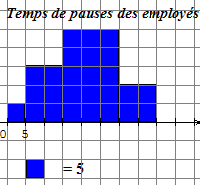
\includegraphics[width=4cm]{images/histo.png}
\end{center}
\end{minipage}
&
\begin{minipage}{11cm}
\begin{enumerate}
  \item Repr�senter la s�rie sous forme de tableau.
  \item D�terminer la m�diane de la s�rie.
\end{enumerate}
\end{minipage}
\end{tabular}


\subsection*{Exercice 3}
 

Maud veut calculer rapidement sa moyenne, ses notes sont:
10 \quad 12 \quad 14 \quad 7.5 \quad 13 \quad 9.5 \quad 11 \quad 15.

Maud enl�ve 10 � chaque note; elle calcule la moyenne $\bar{y}$ des nombres
obtenus puis rajoute 10 pour obtenir sa moyenne.

\begin{enumerate}
  \item Effectuer le calcul de Maud.
  \item Citer la propri�t� utilis�e.
 \end{enumerate}

\subsection*{Exercice 4}

Soient $A$ un point du plan et $\vec{u}$, $\vec{v}$ deux vecteurs.

\enskip

\begin{tabular}{cc}
\begin{minipage}{10cm}
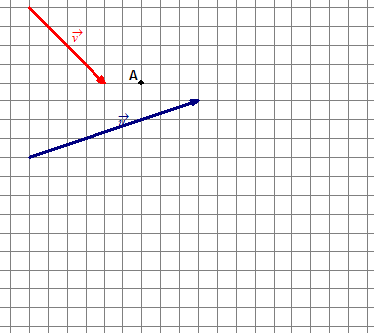
\includegraphics[width=9cm]{images/vec.png}
\end{minipage}
& 
\begin{minipage}{8cm}
\begin{enumerate}
  \item Construire le point $E$ tel que $\overrightarrow{AE}=\dfrac{2}{3}
  \vec{u}$.
\item  Construire le point $F$ tel que $\overrightarrow{AF}=\dfrac{5}{4}
  \vec{v}$.  
 \item Construire le point $G$ tel que $\overrightarrow{AG}=2
 \overrightarrow{AF}-\overrightarrow{AE}$.
 \item Ecrire $\overrightarrow{EF}$ en fonction de  $\vec{u}$ et $\vec{v}$.
 \item Ecrire $\overrightarrow{EG}$ en fonction de  $\vec{u}$ et $\vec{v}$.
 \item En d�duire que les points $E$, $F$ et $G$ sont align�s.
\end{enumerate}
\end{minipage}
\end{tabular}
\end{document}
